\chapter{Riducibilità}

\section{\emph{Many-to-one} reducibility}

Abbiamo in precedenza visto dei procedimenti di ``riduzione'' da un insieme $A$ a $K$ per dimostare,
ad esempio, che se $A$ fosse ricorsivo anche $K$ lo sarebbe. Andiamo ora a definire formalmente la
nostra nozione di riducibilità. Ne esistono tante versioni diverse di questa nozione, noi ne
vediamo una concettualmente semplice che va sotto il nome di $m$-riducibilità. La $m$ sta per
\emph{many-to-one}; esiste ance la riduzione \emph{one-to-one}.

\begin{defn}
    Siano $A,B \subseteq \Nat$. Un insieme $A$ è $m$-riducibile a $B$ ($A \leq_{m} B$) sse
    $\exists f$ totale calcolabile tale che $x \in A \iff f(x) \in B$.
\end{defn}

Si parla di riducibilità perché possiamo ridurre la appartenenza ad $A$ all'appartenenza a $B$.
Per ogni $x$ mi basta calcolare $f(x)$ e vedere se sta in $B$ per sapere automaticamente se $x$
appartiene ad $A$. Nella \emph{one-to-one} reducibility si richiede anche che $f$ sia iniettiva. È una
nozione che troveremo molto simile nella parte di complessità, avremo solo degli ulteriori limiti
sulla complessità di $f$. 

Per dimostrare che $A \leq_{m} B$ devo fare due cose:
\begin{itemize}
    \item per prima cosa devo definire $f: \Nat \to \Nat$ totale calcolabile;
    \item dopodiché va dimostrato che è una buona funzione di riduzione, ovvero va dimostrato il
    $\iff$ della definizione.
\end{itemize}

È un esercizio creativo, cambia per diversi $A$ a $B$. La $m$-riducibilità è un ordine parziale.
Infatti $A \leq_{m} A$, con la funzione identità, e se $A \leq_{m} B$ e $B \leq_{m} C$, allora, componendo le due
funzioni di riduzione, otteniamo una funzione di riduzione da $A$ a $C$:$A \leq_{m} C$. 

Notazione: $A \leq_{m}^{f} B$ se $A$ è riducibile a $B$ attraverso la funzione $f$.

Se $A \leq_{m} B$ e $B \leq_{m} A$ allora scriveremo $A =_{m} B$. Intuitivamente sono equivalenti
dal punto di vista della riducibilità.

La nozione di riducibilità ci dà un'idea di quanto complicato è un problema. Se $A \leq_{m} B$
allora $B$ è tanto difficile quanto lo è $A$. Quanto fine è la mia misurazione dipende dalla potenza
della mia nozione di riducibilità. Se la mia nozione di riducibilità non ha troppe pretese rischio
di passare da un problema ricorsivo ad uno ricorsivamente enumerabile, e di avere molte riduzioni
possibili non molto significative.

Tutti i problemi ricorsivi sono mutuamente riducibili ad esempio. Infatti supponiamo $x \in A \iff
f(x) \in B$. A sto punto se $B$ è ricorsivo ovviamente posso decidere l'appartenenza ad $A$, e
quindi $A$ è ricorsivo. Se invece $B$ è r.e. allora, per lo stesso motivo, anche $A$ risulta essere
r.e.

L'altra implicazione non è vera. È possibile passare da un problema ricorsivo ad uno
ricorsivamente enumerabile. Il minore o uguale ha il significato intuitivo di ``$A$ non è più
difficile di $B$''.

Supponiamo di avere due insiemi ricorsivi non banali. Mostriamo che sono sempre mutuamente
riducibili l'uno all'altro. Dimostriamo solo $A \leq_{m} B$; il verso opposto usa le stesse ipotesi.
Esistono allora $b_{1} \in B$ e $b_{2} \in \comp{B}$. È banale costruire ora $f(x)$ tale che:
\begin{equation*}
    f(x) =
    \begin{cases}
        \case{b_{1}}{se $x \in A$} \\
        \case{b_{2}}{se $x \notin A$}
    \end{cases}
\end{equation*}

È una funzione totale calcolabile? Sì. Vale il sse della definizione di riducibilità? Anche, e si
vede quasi subito. È importante l'ipotesi di non banalità di $A$ e $B$. Non abbiamo usato l'ipotesi di
ricorsività di $B$. Se $B$ è un qualsiasi insieme non banale posso ridurre $A$ a $B$. Senza altre ipotesi
potrei non essere in grado di tornare indietro.

Prendiamo un insieme non ricorsivo come $K$ e supponiamo che $K$ sia riducibile ad $A$. Cosa abbiamo
concluso? Che $A$ non è ricorsivo. Analogamente se $\comp{K} \leq_{m} A$ allora $A$ non è r.e.

Abbiamo infine che $A \leq_{m} B \iff \comp{A} \leq_{m} \comp{B}$.

\section{Completezza}

Passiamo ora alla nozione di completezza. Di solito è relativa ad una classe di problemi. Qua siamo
interessati alla classe dei problemi semidecidibili.
\begin{defn}
    Diciamo che un certo problema $B$ è completo (per i problemi r.e.) se
    \begin{itemize}
        \item $B$ è r.e.
        \item $\forall A$, se $A \in \RE$, allora $A \leq_{m} B$
    \end{itemize}
\end{defn}

Potrei definire la stessa nozione per altre classi di problemi.

Il primo punto che ci interessa è, esistono dei problemi completi? La risposta è sì. Prendiamo ad
esempio $K_{1} = \set{<x,y> \mid \phix(y) \converges}$. È banalmente semidecibile. È completo? Supponiamo
che $A$ sia r.e. Esiste quindi il semidecisore di $A$, $s_{A}$. Supponiamo che sia il programma di
indice $a$ nella mia enumerazione dei programmi: $\phi_{a}(x)$. Quindi $x \in A$ sse $\phia(x) \converges$
sse $<a,x> \in K_{1}$. La funzione $f$ che mi interessa è la funzione che mappa $x$ nella coppia
$<a,x>$ : $x \mapsto <a,x>$.

Ne esistono altri? Si, ad esempio $K$ è completo. Si può dimostrare direttamente. Noi però
dimostreremo che $K \equiv_{m} K_{1}$. È facile vedere che $K \leq_{m} K_{1}$. La mia $f$ è quella tale
che $x \mapsto <x,x>$. Abbiamo che $x \in K \iff \phix(x)\converges \iff <x,x> \in K_{1}$.

La parte $K_{1} \leq_{m} K$ è un pò più tricky. Vogliamo catturare un comportamento puntuale sulla
diagonale. Questo è difficile; possiamo piuttosto catturare un comportamento uniforme che valga
ovunque, e che quindi in particolare valga anche per la diagonale.

Sia $f$ tale che
\begin{equation*}
    f(x,y,z) =
    \begin{cases}
        \case{1}{se $\phix(y) \converges$} \\
        \case{\diverges}{altrimenti}
    \end{cases}
\end{equation*}

Utilizzo ora s-m-n sulla coppia $<x,y>$: esiste $\phi_{s(x,y)}(z)$ con lo stesso comportamento. La mia
funzione $s$ è quella che cerco (questo è il mio claim).

Supponiamo che $(x,y) \in K_{1}$. Allora $\forall z \phi_{s(x,y)}(z) \converges$. In particolare
converge anche sulla diagonale. In particolare $\phi_{s(x,y)}(s(x,y)) \converges$, e qindi $s(x,y) \in
K$. Inoltre $(x,y) \notin K_{1} \implies \forall z \phi_{s(x,y)}(z) \diverges \implies
\phi_{s(x,y)}(s(x,y)) \diverges \implies s(x,y) \notin K$.

Come conseguenza abbiamo che tutti gli insiemi completi sono mutuamente riducibili: $A$ e $B$ completi
$\implies A \equiv_{m} B$.

\section{Insiemi produttivi e creativi}

Cerchiamo ora di dare altre caratterizzazioni degli insiemi completi. Vediamo se hanno delle
proprietà interessanti. Una proprietà curiosa è la creatività.

\begin{defn}
    Sia $A \subseteq \Nat$. $A$ è produttivo se esiste $f$ totale calcolabile, detta funzione di
    produzione, tale che comunque prendo un sottoinsieme $W_{i} \subseteq A$ , si ha che $f(i) \in A
    \setminus W_{i}$.
\end{defn}

Ricordiamo che $W_{i}$ è la numerazione dei sottoinsiemi r.e. basata sul dominio di convergenza
della funzione $i$ della mia numerazione delle funzioni calcolabili.

Cos'è che produce la funzione di produzione? Uno potrebbe essere interessato a dare una
approssimazione r.e. di questi insiemi. Cosa intendiamo? Dare un sottoinsieme di $A$ ricorsivamente
enumerabile. $f$ mi produce una dimostrazione, per ogni approssimazione, dell'incompletezza della
mia approssimazione in funzione dell'algoritmo con cui enumeriamo i programmi. $f$ è unica,
definita a prori dall'insieme $A$. Questo concetto è stato suggerito dai problemi di incompletezza
logica.

C'è una caratterizzazione degli insiemi completi attraverso la produttività.

%\begin{defn}
%    Sia $A \subseteq \Nat$. $A$ è produttivo sse $\exists f$ totale calcolabile tale che $\forall
%    i, W_{i} \subseteq A \implies f(i) \in A \setminus W_{i}$.
%\end{defn}

Possiamo pensare ad $A$ come all'insieme delle formule vere dell'aritmetica. Quando costruiamo un
sistema formale per ragionare sull'aritmetica, ovvero un sistema di assiomi fondamentalmente e le regole
logiche per passare alle conseguenze logiche degli assiomi, avremo, per il teorema di incompletezza,
che ci saranno sempre formule vere che non sono però dimostrabili nel sistema formale.

È una tecnica simile alla diagonalizzazione.

Un insieme produttivo non è, per sua natura, r.e.; altrimenti potrei approssimarlo con l'insieme
stesso.

\begin{defn}
    Un insieme $A \subseteq \Nat$ è creativo se $A$ è r.e. e $\comp{A}$ è produttivo.
\end{defn}

Non tutti gli insiemi produttivi hanno un complementare r.e.

$K$ è un esempio di insieme creativo. Per dimostrarlo ci manca solo da dimostrare che $\comp{K}$ è
produttivo. Questo è semplice però perché la funzione di produzione per $\comp{K}$ è la funzione
identità.

Sia $W_{i} \subseteq \comp{K}$. Dobbiamo dimostrare che $i \in \comp{K}$ e $i \notin W_{i}$.

Per la prima appartenenza andiamo per assurdo. Supponiamo che $i \in K$. Allora $i \in W_{i}$. Ma
essendo $W_{i}$ sottinsieme di $\comp{K}$ si ha $i \in \comp{K}$, il che è assurdo. Quindi $i \in
\comp{K}$.

Per la seconda appartenenza andiamo nuovamente per assurdo. $i \in W_{i} \implies i \in K \implies
\absurd \implies i \notin W_{i}$.

\section{Relazione tra creatività e completezza}

Nota: La seguente è l'ultima dimostrazione richiesta per l'orale.

Da qui in poi verrà usato il simbolo $\leq$ sottintendendo $\leq_{m}$. Vediamo un risultato
importante per gli insiemi produttivi

\begin{thm}
    Un insieme $A \subseteq \Nat$ è produttivo sse $\comp{K} \leq A$.
\end{thm}

Questo implica come corollario che $A$ è creativo sse $A$ è r.e. e $K \leq A$. Di conseguenza
insiemi creativi ed insiemi completi coincidono.

\begin{proof}
    Dimostriamo il primo teorema. Abbiamo i due versi del $\iff$ da dimostrare. Il più semplice dei due è
    quello inverso: $\comp{K} \leq A \implies A$ è produttivo.

    Sia quindi $\comp{K} \leq A$. Sia $f$ la funzione di riducibilità di $\comp{K}$ in $A$. Sappiamo anche che
    $\comp{K}$ è produttivo, con funzione di produzione uguale ad \textit{Id}. L'idea è di ritornare a
    $\comp{K}$ da $A$ attraverso $f$. Dopodiché, utilizzando la funzione di produzione di
    $\comp{K}$,
    troviamo un nuovo elemento che, attraverso alla funzione $f$, sta in $A$ e non in $W_{i}$.

    Ricordiamo che la controimmagine di una insieme $A$ attraverso una funzione $f$ è definita come
    l'insieme $f^{-1}(A) = \set{x \mid f(x) \in A})$.

    Consideriamo $f^{-1}(W_{i})$, la controimmagine di $W_{i}$ via $f$. Abbiamo che sicuramente
    $f^{-1}(W_{i}) \subseteq \comp{K}$ e che è r.e. L'indice di $f^{-1}(W_{i})$ può essere calcolato
    in maniera effettiva attraverso una funzione totale calcolabile $h$.  Abbiamo quindi che
    corrisponde a $W_{h(i)}$. Pensiamo alla funzione $\phii(f(x)) = \phi_{h(i)}(x)$ per s-m-n. Dove
    sta $h(i)$?  Sta in $\comp{K}$ ma non in $f^{-1}(W_{i})$, essendo $\comp{K}$ produttivo con
    funzione di produzione uguale a \textit{Id}. Passando quindi, attraverso $f$, al corrispondente
    in $A$ (ovvero $f(h(i))$) abbiamo che sta in $A$ ma non in $W_{i}$. Quindi $A$ è produttivo.

    La dimostrazione poteva essere fatta con un altro insieme produttivo. In particolare, se $B$ è
    produttivo e $B \leq A$ allora $A$ è produttivo.

    Passiamo ora al verso opposto: $A$ produttivo $\implies \comp{K} \leq A$.

    Sia $A$ produttivo e sia $f$ la funzione di produzione per $A$. Vado alla ricerca di $W_{s(i)}$
    tale che:
    \begin{equation*}
        W_{s(i)} =
        \begin{cases}
            \case{\{f(s(i))\}}{se $i \in K$} \\
            \case{\emptyset}{se $i \in \comp{K}$}
        \end{cases}
    \end{equation*}

    Non sappiamo, per ora, se esiste $s$; supponiamo però di poterla definire. Per dimostrare la
    sua esistenza ricorreremo al teorema del punto fisso.

    Vogliamo dimostrare che $i \in \comp{K}$ sse $f(s(i)) \in A$. Supponiamo che $i \in \comp{K}$.
    Allora $W_{s(i)} = \emptyset \subseteq A$. Posso applicare la produttività e quindi concludere
    che $f(s(i)) \in A$.

    Supponiamo che $i \in K$. Allora $W_{s(i)} = \{f(s(i))\}$. Supponiamo per assurdo che $f(s(i)) \in A$.
    Allora $W_{s(i)} \subseteq A$. Sfruttando la produttività avremmo che $f(s(i)) \in A$ e che
    $f(s(i)) \notin W_{s(i)}$. Ma questo è assurdo. Perciò $f(s(i)) \notin A$.

    La dimostrazione è incompleta, manca la dimostrazione dell'esistenza di $s$. Ci serve il secondo
    teorema di ricorsione. Partiamo da $g(i,z,x)$ tale che:
    \begin{equation*}
        g(i,z,x) =
        \begin{cases}
            \case{1}{se $\phi(i) \converges \land$ $x = f(z)$} \\
            \case{\diverges}{se $\phii(i) \diverges$}
        \end{cases}
    \end{equation*}
    
    Per s-m-n esiste $h(i,z)$ tale che $\phi_{h(i,z)}(x)$ ha lo stesso comportamento. Esiste ora $s$ tale che
    $\forall i, \phi_{s(i)} = \phi_{h(i,s(i))}$. Abbiamo quindi che
    \begin{equation*}
        \phi_{s(i)}(x) = \phi_{h(i,s(i))}(x) = g(i,s(i),x) =
        \begin{cases}
            \case{1}{se $\phii(i) \converges \land$ $x = f(s(i))$} \\
            \case{\diverges}{se $\phii(i) \diverges$}
        \end{cases}
    \end{equation*}
\end{proof}

\begin{proof}
    Dimostriamo il corollario. Sia $A$ creativo. Allora $A$ è r.e. e $\comp{A}$ è produttivo. Allora
    $\comp{K} \leq \comp{A}$. Ma questo implica che $K \leq A$.

    Sia $A$ r.e. e completo. Allora $K \leq A$. Allora $\comp{K} \leq \comp{A}$, quindi $\comp{A}$ è
    produttivo, di conseguenza $A$ è creativo.
\end{proof}

\section{Insiemi r.e. non completi}

Supponiamo di avere un insieme $A$ r.e. Vogliamo dimostrare che $A$ non è ricorsivo. Posso condurre
questa dimostazione sempre dimostrando che $K \leq A$? Limitatamente agli insiemi creativi/completi
allora sì. Il punto è, esiste un insieme r.e. non creativo? Questo va sotto il nome di problema di
Post. È rimasto aperto per un certo numero di anni e veniva considerato un problema difficile.  È
un analogo del problema $\NPClass$ vs $\PClass$. Nella teoria della complessità però si sà molto di meno. È più
facile per un insieme r.e. essere completo che il contrario.

Per rispondere a questa domanda abbiamo bisogno di due risultati intermedi.

\begin{thm}
    Sia $A$ un insieme r.e. infinito. Allora esiste $B$ ricorsivo infinito sottoinsieme di $A$.
\end{thm}
\begin{proof}
    Una caratterizzazione degli insiemi ricorsivi è che sono enumerabili in maniera crescente. Se
    prendo l'enumerazione $f$ di $A$ e la ``taglio'' in pezzetti crescenti e li uso per definire la
    mia enumerazione di $B$ ho che questa è crescente, e quindi $B$ è ricorsivo infinito. 

    Più precisamente, la mia enumeraziona $g$ di $B$ sarà fatta nel modo seguente, se $f$ è la mia
    enumerazione di $A$: $g(0) = f(0)$ e $g(x+1) = f(\mu y. f(y) \geq g(x))$.
\end{proof}

\begin{thm}
    Sia $A$ un insieme ricorsivo infinito. Allora $\exists B$ r.e. non ricorsivo tale che $B \subseteq
    A$.
\end{thm}
\begin{proof}
    Consideriamo una funzione di enumerazione $f$ per $A$ iniettiva. Consideriamo l'insieme $B$ così
    definito:
    \begin{equation*}
        B = \set{f(i) \mid i \in K}
    \end{equation*}

    Abbiamo che $B$ è sottoinsieme di $A$ e che $B$ è r.e. non ricorsivo. Infatti se $B$ fosse
    decidibile lo sarebbe anche $K$. In particolare, abbiamo che $i \in K \implies f(i) \in B$.
    Viceversa essendo $f$ iniettiva non è possibile che un elemento $i \notin K$ venga mappato da
    $f$ in un elemento $f(i) \in B$. Di conseguenza $i \notin K \implies f(i) \notin B$.
\end{proof}

Se vediamo l'estrazione di sottoinsiemi come un'operazione di focalizzazione possiamo focalizzarci
su insiemi di complessità desiderata 

\begin{figure}[h]
    \centering
    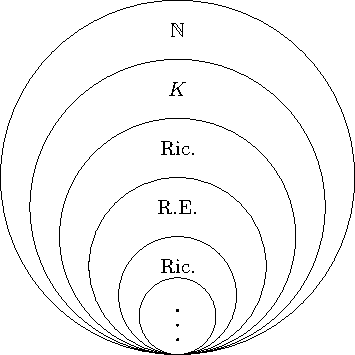
\includegraphics{img/SetsResolution.pdf}
    \caption{Focalizzazione su insiemi}
\end{figure}

%Noi abbiamo intrapreso questo discorso perché cercavamo un insieme r.e. non completo. 
Una proprietà interessante degli insiemi produttivi è che ogni insieme produttivo contiene un
sottoinsieme r.e. infinito.

\begin{thm}
    Sia $A \subseteq \Nat$ produttivo. Allora $\exists B$ r.e. infinito tale che $B \subseteq A$.
\end{thm}

È una proprietà cruciale che ci serve perché costruiremo un insieme infinito che non contiene
alcun sottoinsieme r.e. In pratica abbiamo un insieme tale che qualsiasi suo sosttoinsieme infinito
è talmente caotico da non essere nemmeno r.e.

\begin{proof}
    Per la dimostrazione useremo la produttività. Proviamo ad approssimare $A$. Inizieremo con l'insieme
    vuoto. Per la produttività esiste $a \in A$. Ora nella mia approssimazione includo pure $a$. Per
    produttività esiste $a' \in A$ fuori dalla mia approssimazione, e continuo così all'infinito. Questo
    procedimento è costruttivo e mi crea la mia approssimazione r.e. di $A$.

    Questo procedimento ha un analogo con il tentativo di approssimare l'insieme delle conseguenze
    di un insieme di assiomi. Per l'incompletezza esiste una formula che non è dimostrabile dal mio
    sistema formale. A questo punto potrei aggiungere la validità di questa formula al mio sistema
    formale e crearne uno nuovo. Ma a questo punto ho un nuovo sistema formale, e il ragionamento
    precedente si applicherebbe identicamente. Quindi non potrò mai avere un insieme che contenga
    tutte le conseguenze dei miei assiomi.

    Vogliamo dimostrare che $W_{h(i,a)} = W_{i} \cup {a}$. Più precisamente vogliamo dimostrare che
    esiste un modo effettivo per calcolare un insieme r.e. ottenibile mediante estensione di $W_{i}$
    con $a$. $W_{h(i,a)}$ è il dominio di una certa funzione $\phi_{h(i,a)}$. Vogliamo quindi che
    $\phi_{h(i,a)}(x) = g(i,a,x) = \phii(x)|(x = a)$. In pratica voglio che converga se $x = a$ oppure se
    $x$ fa parte del dominio di $\phii$. $g$ è effettivamente calcolabile e ho quindi un metodo effettivo
    per calcolare $W_{h(i,a)}$ ogni volta.

    Possiamo ora costruire la mia sequenza di approssimazione. $W_{m} = \emptyset$. Sia $s$ la
    funzione di produzione per $A$. Ho che $s(m) \in A \setminus W_{m}$. Passo quindi a
    $W_{h(m,s(m))=m_{1}} = \set{s(m)}$. La mia seconda approssimazione sarà $W_{h(m_{1},s(m_{1}))} =
    \set{s(m),s(m_{1})}$.

    Se definiamo $\textit{next}(x) = h(x,s(x))$ possiamo definire $g(x) = next^{x}(m_{0})$ e abbiamo
    che $B$ è uguale al codominio di $g$.
\end{proof}

\subsection{Complessità di Kolmogorov}

Se noi vogliamo trasmettere un'informazione, diciamo il numero $n$, abbiamo due modi per farlo: uno
è trasmettere direttamente $n$, ad esempio con la sequenza di bit che rappresnta $n$, che ha un
costo che dipende da $n$; un'altra possibilità è trasmettere un modo per costruire $n$. Ad esempio un
algoritmo.

In particolare, immaginiamo un programma $i$ tale che $\phii(0) = n$. Posso trasmettere direttamente
$i$. Qual è più conveniente? Intuitivamente quello più piccolo. Confronto $i$ con $n$. Se $i$ è più
piccolo trasmetto $i$, altrimenti trasmetto $n$.

\begin{defn}
    La complessità di Kolmogorov di $n$, $K(n)$, è il minimo $i$ tale che $\phii(0) = n$ (=
    $\min\set{i \mid \phii(0) = n}$).
\end{defn}

È una astrazione di una problematica reale legata alla comprimibilità delle informazioni.

Il mio confronto è tra $n$ e $K(n)$.

\subsection{Numeri random}

\begin{defn}
    $n \in \Nat$ è un numero random se $n \leq K(n)$.
\end{defn}

Dobbiamo pensare a $n$ come alla sua espansione decimale: una stringa di bit.

Perché usiamo la nozione di \textit{Random} per descrivere questa caratteristica? Perché è una
idea del concetto. Se ci fosse una grande regolarità nella stringa per $n$ è chiaro che posso creare
un programma piccolino che lo generi. Si parla di dati lawful o lawless. I dati che seguono una
regola non saranno random. Se sono random sono talmente disordinati che non riesco a dare nessun
metodo generativo più breve dei dati stessi. È un approccio formale alla nozione di random legata
alla comprimibilità del dato.

Come l'abbiamo vista la nostra nozione di ``casualità'' dipende dalla nostra enumerazione dei programmi.
Per numeri grandi però non dovrebbe cambiare niente se cambia l'enumerazione.

Un'altra questione è che la nostra nozione di random va bene per sequenze finite. Noi in generale
vorremmo idealmente una nozione che valga per sequenze infinite. In questo contesto però ci è
sufficiente.

La randomicità di un numero è decidibile? È semidecidibile? Potrei pensare di fare una ricerca
limitata ad $n$ per un programma che genera $n$. Il problema è che le mie funzioni sono parziali
calcolabili, potrebbero divergere. Quindi sembrerebbe che la risposta sia no.

Cosa possiamo però semidecidere? Se un numero non è random. Se $\Rand$ è l'insieme dei numeri random
allora abbiamo che $\comp{\Rand}$ è semidecidibile. La nostra congettura è che $\Rand$ non sia nemmemno
semidecidibile.

Abbiamo un altro modo per dimostrare quanto detto su $\comp{\Rand}$, oltre al lanciare in parallelo
tutti i $\phii$ e aspettare che uno di essi termini. Lanciamo $\phii(0)$ e vediamo se è uguale a
$n$. Se $\phii(0) = n$ e $i < n$ allora restituisco $n$, altrimenti divergo. Questa funzione
$g(<i,n>)$ è una funzione di numerazione parziale che dà fuori numeri che non sono random. Prima o
poi tutti i numeri non random verranno enumerati.

Il nostro claim è che l'insieme dei numeri random non è produttivo.

Vogliamo dimostrare che $\Rand$ non è produttivo. Lo dimostriamo facendo vedere che $\Rand$ non contiene
nessun sottoinsieme r.e. infinito.

Noi dimostriamo ciò dimostrando che in $\Rand$ non ci sia nessun sottoinsieme ricorsivo infinito.
Grazie ai risultati dimostrati in precedenza è equivalente.

Supponiamo, per assurdo, che $A$ sia ricorsivo e che $A \subseteq \Rand$. Definiamo $g(i,x) = \mu n, n \in A$
e $n > i$. L'idea è che $A$ è ricorsivo, e quindi possiamo decidere $n \in A$, e possiamo andare alla
ricerca del più piccolo $n$ maggiore di $i$. Questa funzione è calcolabile e per s-m-n abbiamo che
possiamo calcolarla con $\phi_{h(i)}(x)$. 

Esitste $p$ tale che $\phi_{p}(x) = \phi_{h(p)}(x) = \mu n, n \in A$ e $n > p$, per il teorema del
punto fisso. Ora mi chiedo $\phip(0)$ è random? Dovrebbe essere random, dato che l'output sta in $A
\subseteq \Rand$. Ma al tempo stesso $\phip(0)$ è generato da $p$ e, per costruzione, $p < \phip(0)$. E
quindi sarebbe non random. Assurdo.

Questa parte è legata al paradosso di Berry.

Un insieme che non contiene insiemi r.e. infiniti è detto immune e il suo complementare è detto
semplice.

Abbiamo quindi che l'insieme dei numeri random non è produttivo. Di conseguenza l'insieme $\comp{\Rand}$ 
è r.e. non ricorsivo e non creativo, ovvero non completo.
